\chapter{Future Work} \label{fw}


The future work for this PhD will look at different techniques to finding stopping points. This will look at adapting stopping methods so that they do not \textbf{depend on ranked document collections}. This makes absolute sense as a study is never considered to be more relevant than any other. Instead, they are considered to be relevant or non relevant. 


\section{Rank-based methods to Stopping}

An area that could be further expanded on is the use of using the similarity score in the initial rankings as a basis for comparing documents. In novel work section \ref{simScoreMethod} we examined a technique that uses the top document as the pseudo document for comparing subsequent documents. To improve the accuracy of the pseudo point we could try using different intervals in the rankings and taking average over a set of points:


\begin{figure}[H]
\center
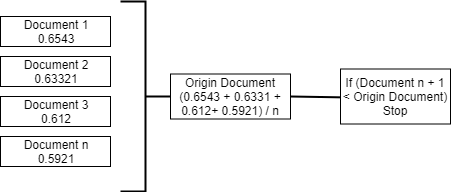
\includegraphics[height=4cm]{figures/originMethod.png}
\caption{Calculating Origin Average}
\end{figure}

The \% difference between document $n+1$ and the pseudo document would still be used to derive the stopping point.

This approach has the advantage of taking into consideration variability in the quality of the rankings. It also has the advantage of being entirely unsupervised and does not require us to sample the initial document collection. 

A further development of this method is to create an pseudo document using the document abstract text:

\begin{figure}[H]
\center
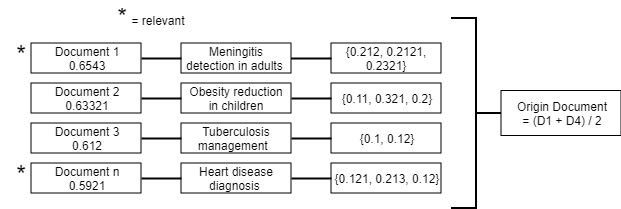
\includegraphics[height=4cm]{figures/origin2.png}
\caption{Generating Origin vector using document abstract}
\end{figure}


We have further developed the method in that we are using the top $n$ documents to calculate an average document vector by using the content of the document. We can then use vector similarity comparisons such as euclidean distance and cosine similarity to compare the origin document vector to further documents down the rankings.

This method can be tweaked and optimized by standard by applying standard text processing/NLP techniques:

\begin{itemize}
  \item Using Word2Vec to represent abstract features
  \item Language modelling abstract features, trying out different NGram sizes
  \item Pre-processing of a abstracts
  
\end{itemize}

Finally we can use the work in \ref{automatic_f_t_r} as part of this method by extracting further useful information from the full texts. This information could be used to expand the content of the abstract as-well act as a separate source for further information for finding a stopping point.


\begin{figure}[H]
\center
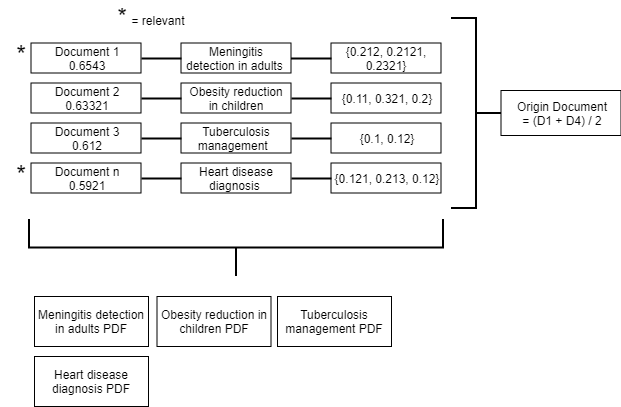
\includegraphics[height=7cm]{figures/origin3.png}
\caption{Generating Origin vector using document abstract and text}
\end{figure}


Another method to stopping that could be applied is implementing a classifier. We would still look to use the abstracts as training data for relevant and non-relevant documents. This method would assume we take a sample set of documents as our training data. This training data would then be used to build a classifier to determine if the rest of the documents are relevant or non relevant. We can infer the expected number of relevant documents from the sample and make the assumptions about how many we would need to find to attain a reliability score of 95\%.


\section{Forest Plot Approaches to Stopping}

Trying to look at different papers that answer the same question is difficult, especially when these papers come to different conclusions \cite{forestplots}. A forest plot takes all of the relevant information asking the same question, extracts the relevant statistical data and displays it on a single axis. 

Each study within the forest plot will carry a level of importance for how much information it contains. Studies that contain more participants will carry a greater weighting in the decision making. The size of the rectangle in the forest plot indicates with importance of the study.

Studies also carry upper and lower bounded confidence intervals of 95\%. Studies with a lower range between confidence intervals are considered more reliable sources of information. Confidence intervals in the forest plot with longer lines with have less influence on the pooled result (diamond).


\begin{figure}[H]
\center
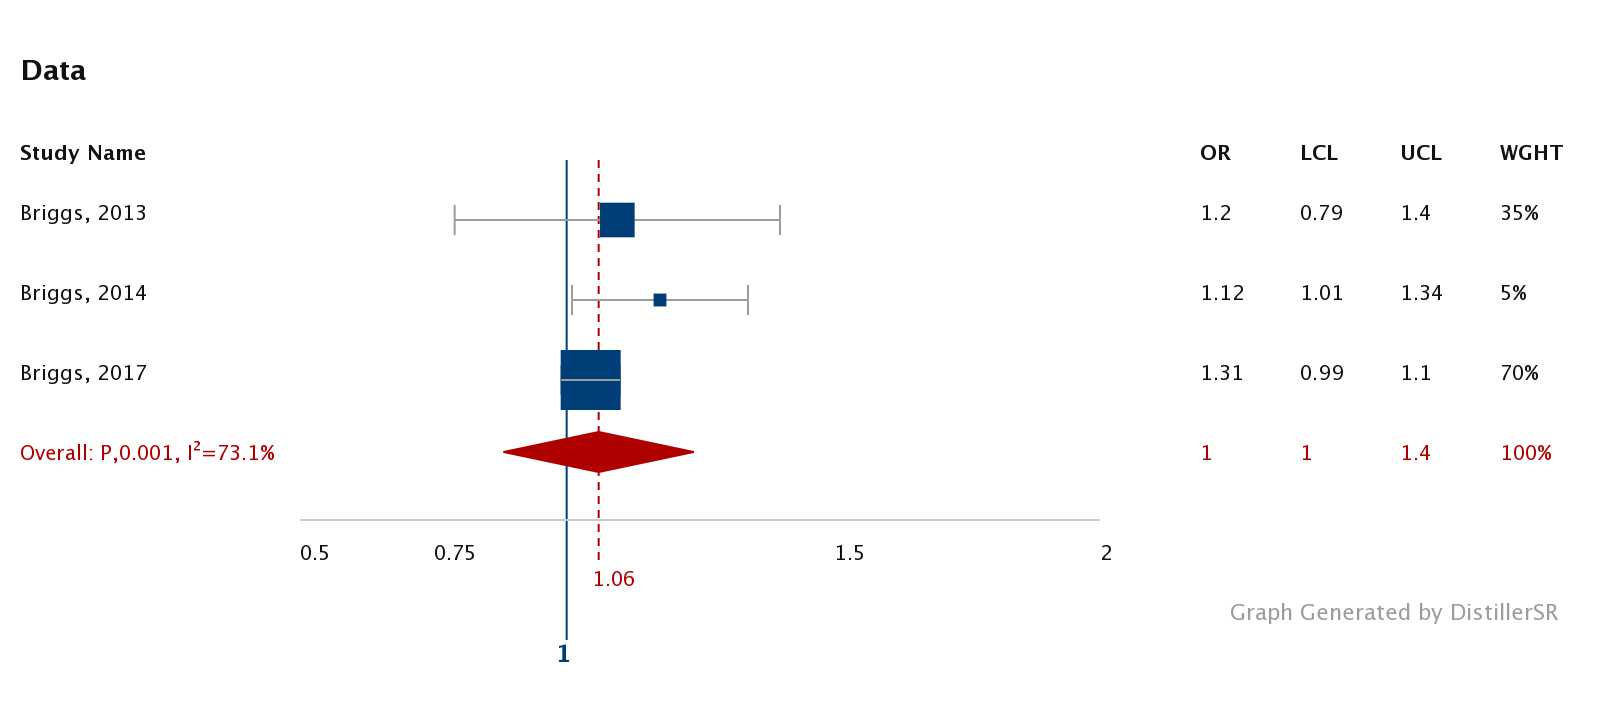
\includegraphics[height=5cm]{figures/forest.png}
\caption{Example Forest plot}
\end{figure}


A stopping method could be developed that uses the meta data from these forest plots to make a decision. Once the pooled result does not change significantly after looking at more studies it could be assumed a decision can be made. Therefore the approach could be assembled as follows:

\begin{enumerate}

\item{Start looking at studies and extracting meta data}
\item{Add meta data to forest plot}
\item{Update pooled result}
\item{Determine weight of change between old and new pooled result}
\item{Repeat steps 1 to 4 and stop when result stops changing}

\end{enumerate}

The challenge would be finding appropriate time to conclude that the pooled result has stopped changing. The task of extracting the meta data could also be modelled as a separate information extraction problem. 





\section{Gnatt Chart} \label{gnatt}


\begin{figure}[H]
\center
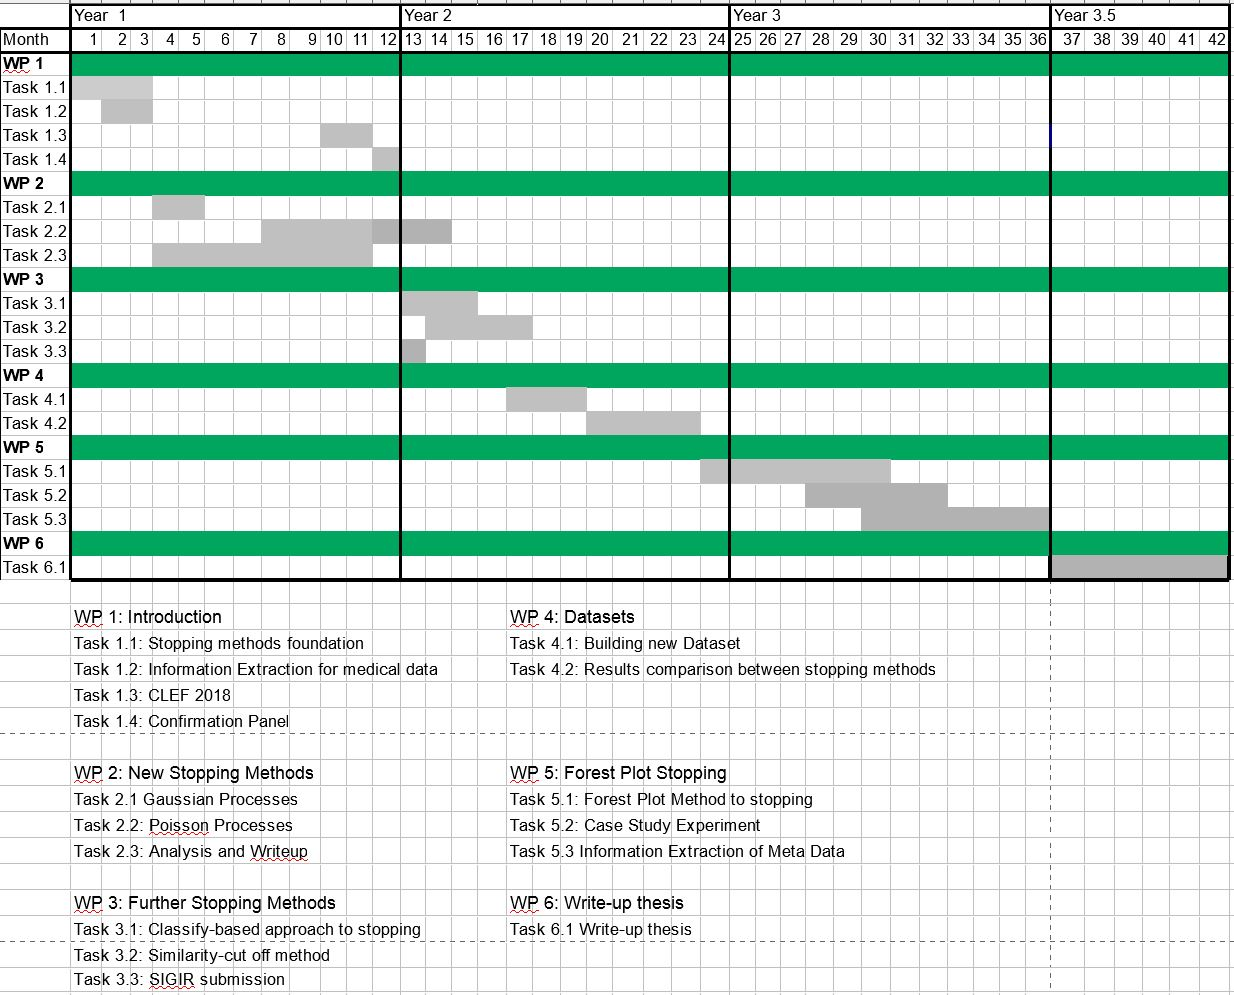
\includegraphics[height=13cm]{figures/gnatt_chart2.jpg}
\caption{Gnatt Chart}
\end{figure}

Initial work focused on background reading around stopping points as well as exploring other ideas as for applying text processing within systematic reviews. Existing approaches to stopping were looked at and evaluated using a new dataset. We submitted some work for the 2018 CLEF conference and attended and presented the work.

We applied a curve fit approach and a Guassian process approach to stopping. Finding the curve showed some promise, but was not flexible in allowing us to specify a desired level of recall. We discovered a GP was not suitable due us being able to infer the distribution of our data already.  An idea that stemmed from using a GP was a Poisson process. It was discovered a non homogeneous Poisson process could be suitable to our problem due to its focus on having variable rate. We applied the NHPP and found results to show promise, but limited due to the variance in quality between topics in the dataset. These results were then written up and compared to previous stopping methods.

Future work will expand on the stopping methods. We will apply a classifier based approach to stopping and look at how additional information can be used strengthen the quality of the dataset rankings. We would first like to map the ranking sets back to the abstracts and use this information predict a stopping point. We would also like to expand this further by using information from the full texts for the same purpose. We would like to further refine the work on the Poisson process approach and submit to SIGIR 2019.

We would also like to expand the datasets so that we have a more robust and general way of testing. The information presented in the current data rankings is variable. We would like these to be consistent. We could also build our own dataset by using the cochrane data and mapping the information back to PubMed.

Another approach that we will apply is using the forest plots as a way for finding a stopping point. We will first attempt to extract this forest plot information from the sample reviews. This approach would work by descending down the rankings until a relevant document has been found. We would update our forest plot with this information and continue to descend down the rankings. The forest plot would keep getting updated until we can make a decision that a stopping point has been found. As as further incentive behind this idea we would also like to apply this approach within a real systematic review process and examine the effectiveness of the strategy. The process of extracting the meta data for updating the forest plot could also be included as an information extraction problem.

The final six months have been reserved for writing up, as this PhD is funded for 3.5 years.
